% !TEX root = thesis.tex
%%%%%%%%%%%%%%%%%%%%%%%%%%%%%%%%%%%%%%%%%%%%%%%%%%%%%%%%%%%%%%%%%%%%
% Results
%%%%%%%%%%%%%%%%%%%%%%%%%%%%%%%%%%%%%%%%%%%%%%%%%%%%%%%%%%%%%%%%%%%%

\chapter{Results}
  \label{sec:res}

\section{Implementation of FracMinHash to obtain phylogenetic outlines}
To evaluate several aspects of FracMinHash, a Java implementation called
\texttt{fmhdist} was created in the context of this thesis. This tool has four
main functions that are described in the following.

\subsection*{\texttt{fmhdist sketch}}

\texttt{fmhdist sketch} takes a list of paths to a sequence file and calculates
the FracMinHash sketch for each sequence. The user can set the $k$-mer size $k$
(defaults to $21$), the scaling parameter $s$ (defaults to $2000$), the hash
function (defaults to \texttt{farm}) and the random seed for the hash function
(defaults to $42$). The user can also specify the output path and weither or not
they want to receive the hash coordinates for each sketch.

\subsection*{\texttt{fmhdist dist}}

\texttt{fmhdist sketch} takes a list of paths to sketch files and calculates the
distance based on the estimated Jaccard index, the distance based on the
estimated containment index
\cite{heraDebiasingFracMinHashDeriving2023,irberLightweightCompositionalAnalysis2022}
and the Mash distance based on the estimated Jaccard index
\cite{ondovMashFastGenome2016}. The distance matrices are stored as a Nexus file
and can be imported in tools such as SplitsTree 6 to obtain the phylogenetic
outline. \todo{add outline generation if applicable}

\subsection*{\texttt{fmhdist db}}

\texttt{fmhdist db} takes a list of NCBI accession codes and creates a reference
dabatase in SQLite format. This database contains the sketches for each taxon
listed in the input as well as the full taxonomic tree that includes those taxa.
If multiple accession codes point to the same taxon, only the first is inserted
in the database. For the sketching, the user has the same choice of parameters
as for \texttt{fmhdist sketch}.

\subsection*{\texttt{fmhdist ref-dist}}

\texttt{fmhdist ref-dist} takes a reference database either as produced by
\texttt{fmhdist db} or as a list of sketches, a set of query sketches and a
threshold. For each query sketch, the pairwise distance based on the Jaccard
estimation is calculated. Those reference sequences that have a distance below
the threshold to any of the query sequences are included in a final pairwise
distance calculation. This works identically to the \texttt{fmhdist dist}
command.


\section{Phylogenies generated for dataset A} 
The trees and outlines generated by \texttt{fmhdist} and \texttt{mashtree},
respectively, and SplitsTree 6
\cite{husonApplicationPhylogeneticNetworks2006,bagciMicrobialPhylogeneticContext2021}
for dataset A generally represent the clade association and the relationships
between clades well. All included taxa are clustered with their corresponding
clade members
\cite{abadPhytophthoraTaxonomicPhylogenetic2023a,yangExpandedPhylogenyGenus2017}.

The dataset also includes several taxa that are represented by multiple
different sequences. This relationship can also be read from the produced trees
and outlines.

\subsection*{Trees}
The tree that was calculated using the re-computed Mash distance for dataset
A is depicted in Figure~\ref{fig:mandalMashTree}. Clade clusters are well
defined and in line with literature
\cite{abadPhytophthoraTaxonomicPhylogenetic2023a,yangExpandedPhylogenyGenus2017}.
Using Newick notation, this tree indicates the following topology: 

\texttt{(((((1, 2), 4), 5), (((7, 3), 6), 8)), 10)}

We can see that the relationships of the inner clades 1, 2 and 4 are in line
with literature, the clades 3, 6, 7 and 8 form a monophyletic group which is not
in line with literature.
\cite{abadPhytophthoraTaxonomicPhylogenetic2023a,yangExpandedPhylogenyGenus2017}.

\begin{figure}
  \centering
  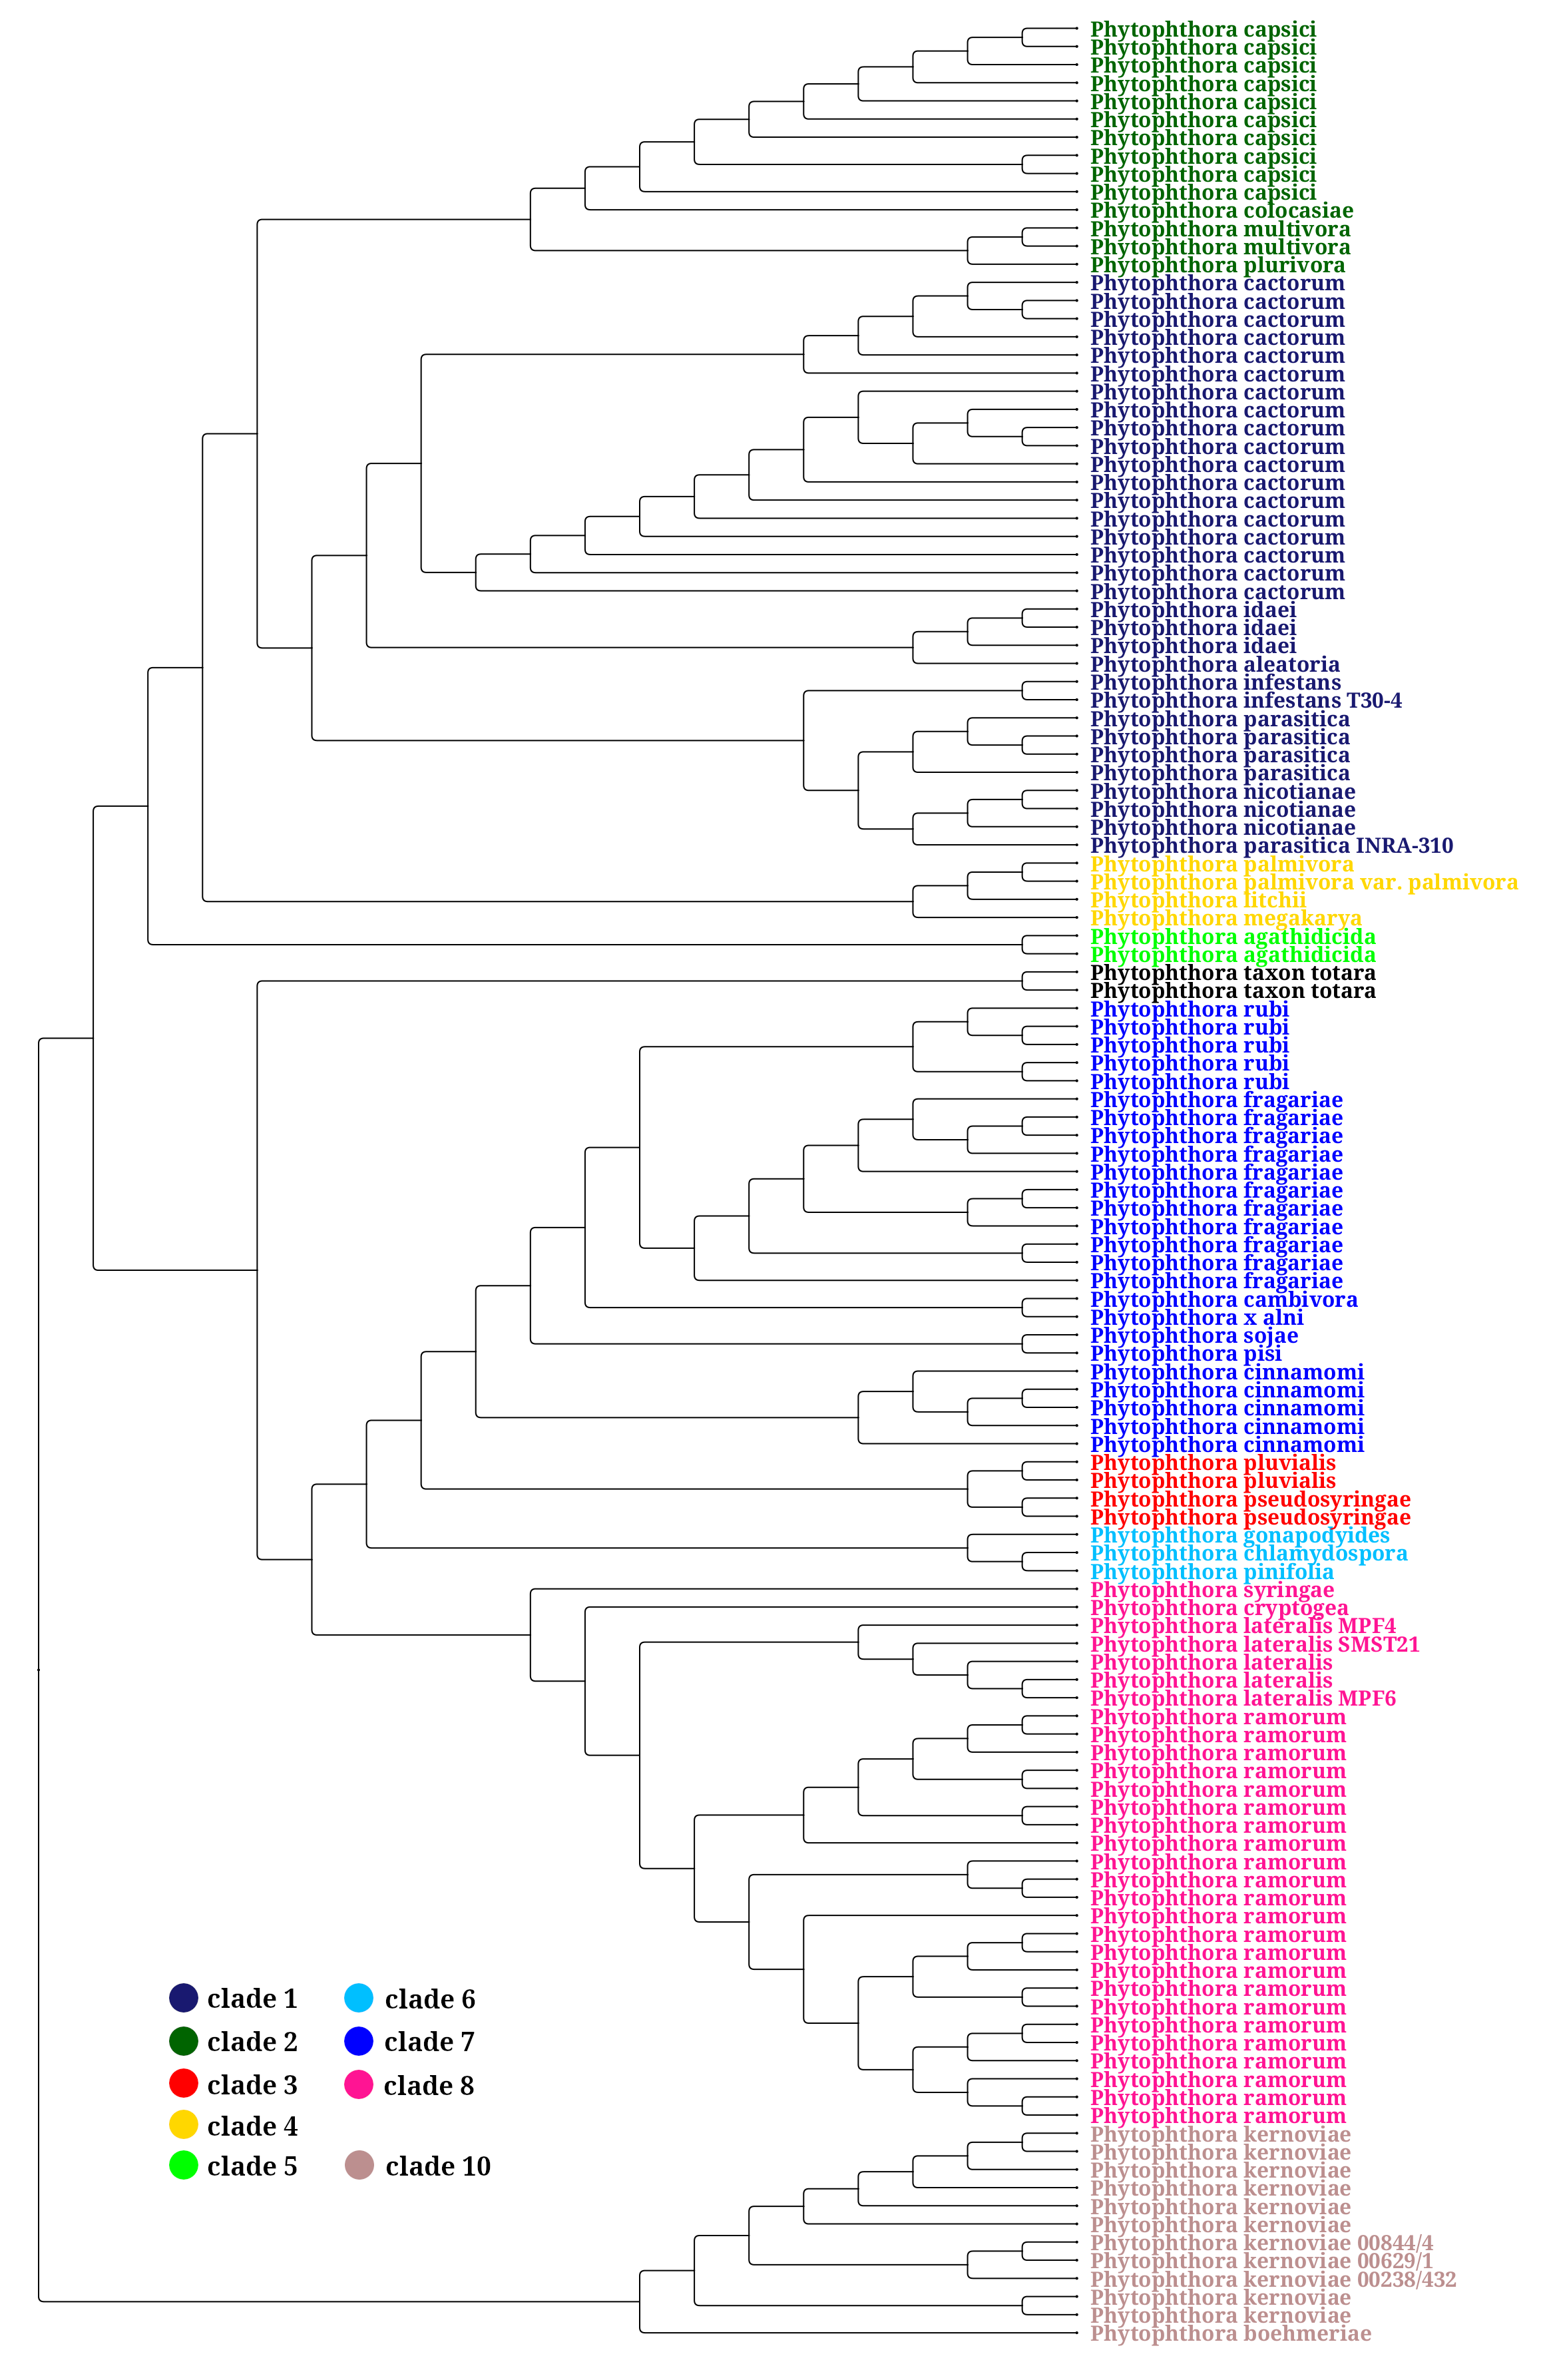
\includegraphics[width=1.0\textwidth]{figures/mashtree_mandal_tree_k21_s2000.png}
  \caption{Phylogenetic tree based on distances of dataset A calculated with
  \texttt{mashtree}
  \cite{ondovMashFastGenome2016,katzMashtreeRapidComparison2019}. Taxa are
  colored according to clade membership
  \cite{abadPhytophthoraTaxonomicPhylogenetic2023a}. The tree is rooted with
  clade 10 as outputgroup.}
  \label{fig:mandalMashTree}
\end{figure}

The tree that was calculated using the FracMinHash distance for dataset A is
depicted in Figure~\ref{fig:mandalFmhdistTree}. Again, clade clusters are well
defined and in line with literature.
Using Newick notation, this tree indicates the following topology:

\texttt{(((((1, 2), 4), 5), (3, ((6, 7), 8))), 10)}

Again, the relationships of the clades 1, 2 and 4 are in line with literature
\cite{abadPhytophthoraTaxonomicPhylogenetic2023a,yangExpandedPhylogenyGenus2017}.
the clades 3, 6, 7 and 8 form a monophyletic group which is not in line with
literature.

\begin{figure}
  \centering
  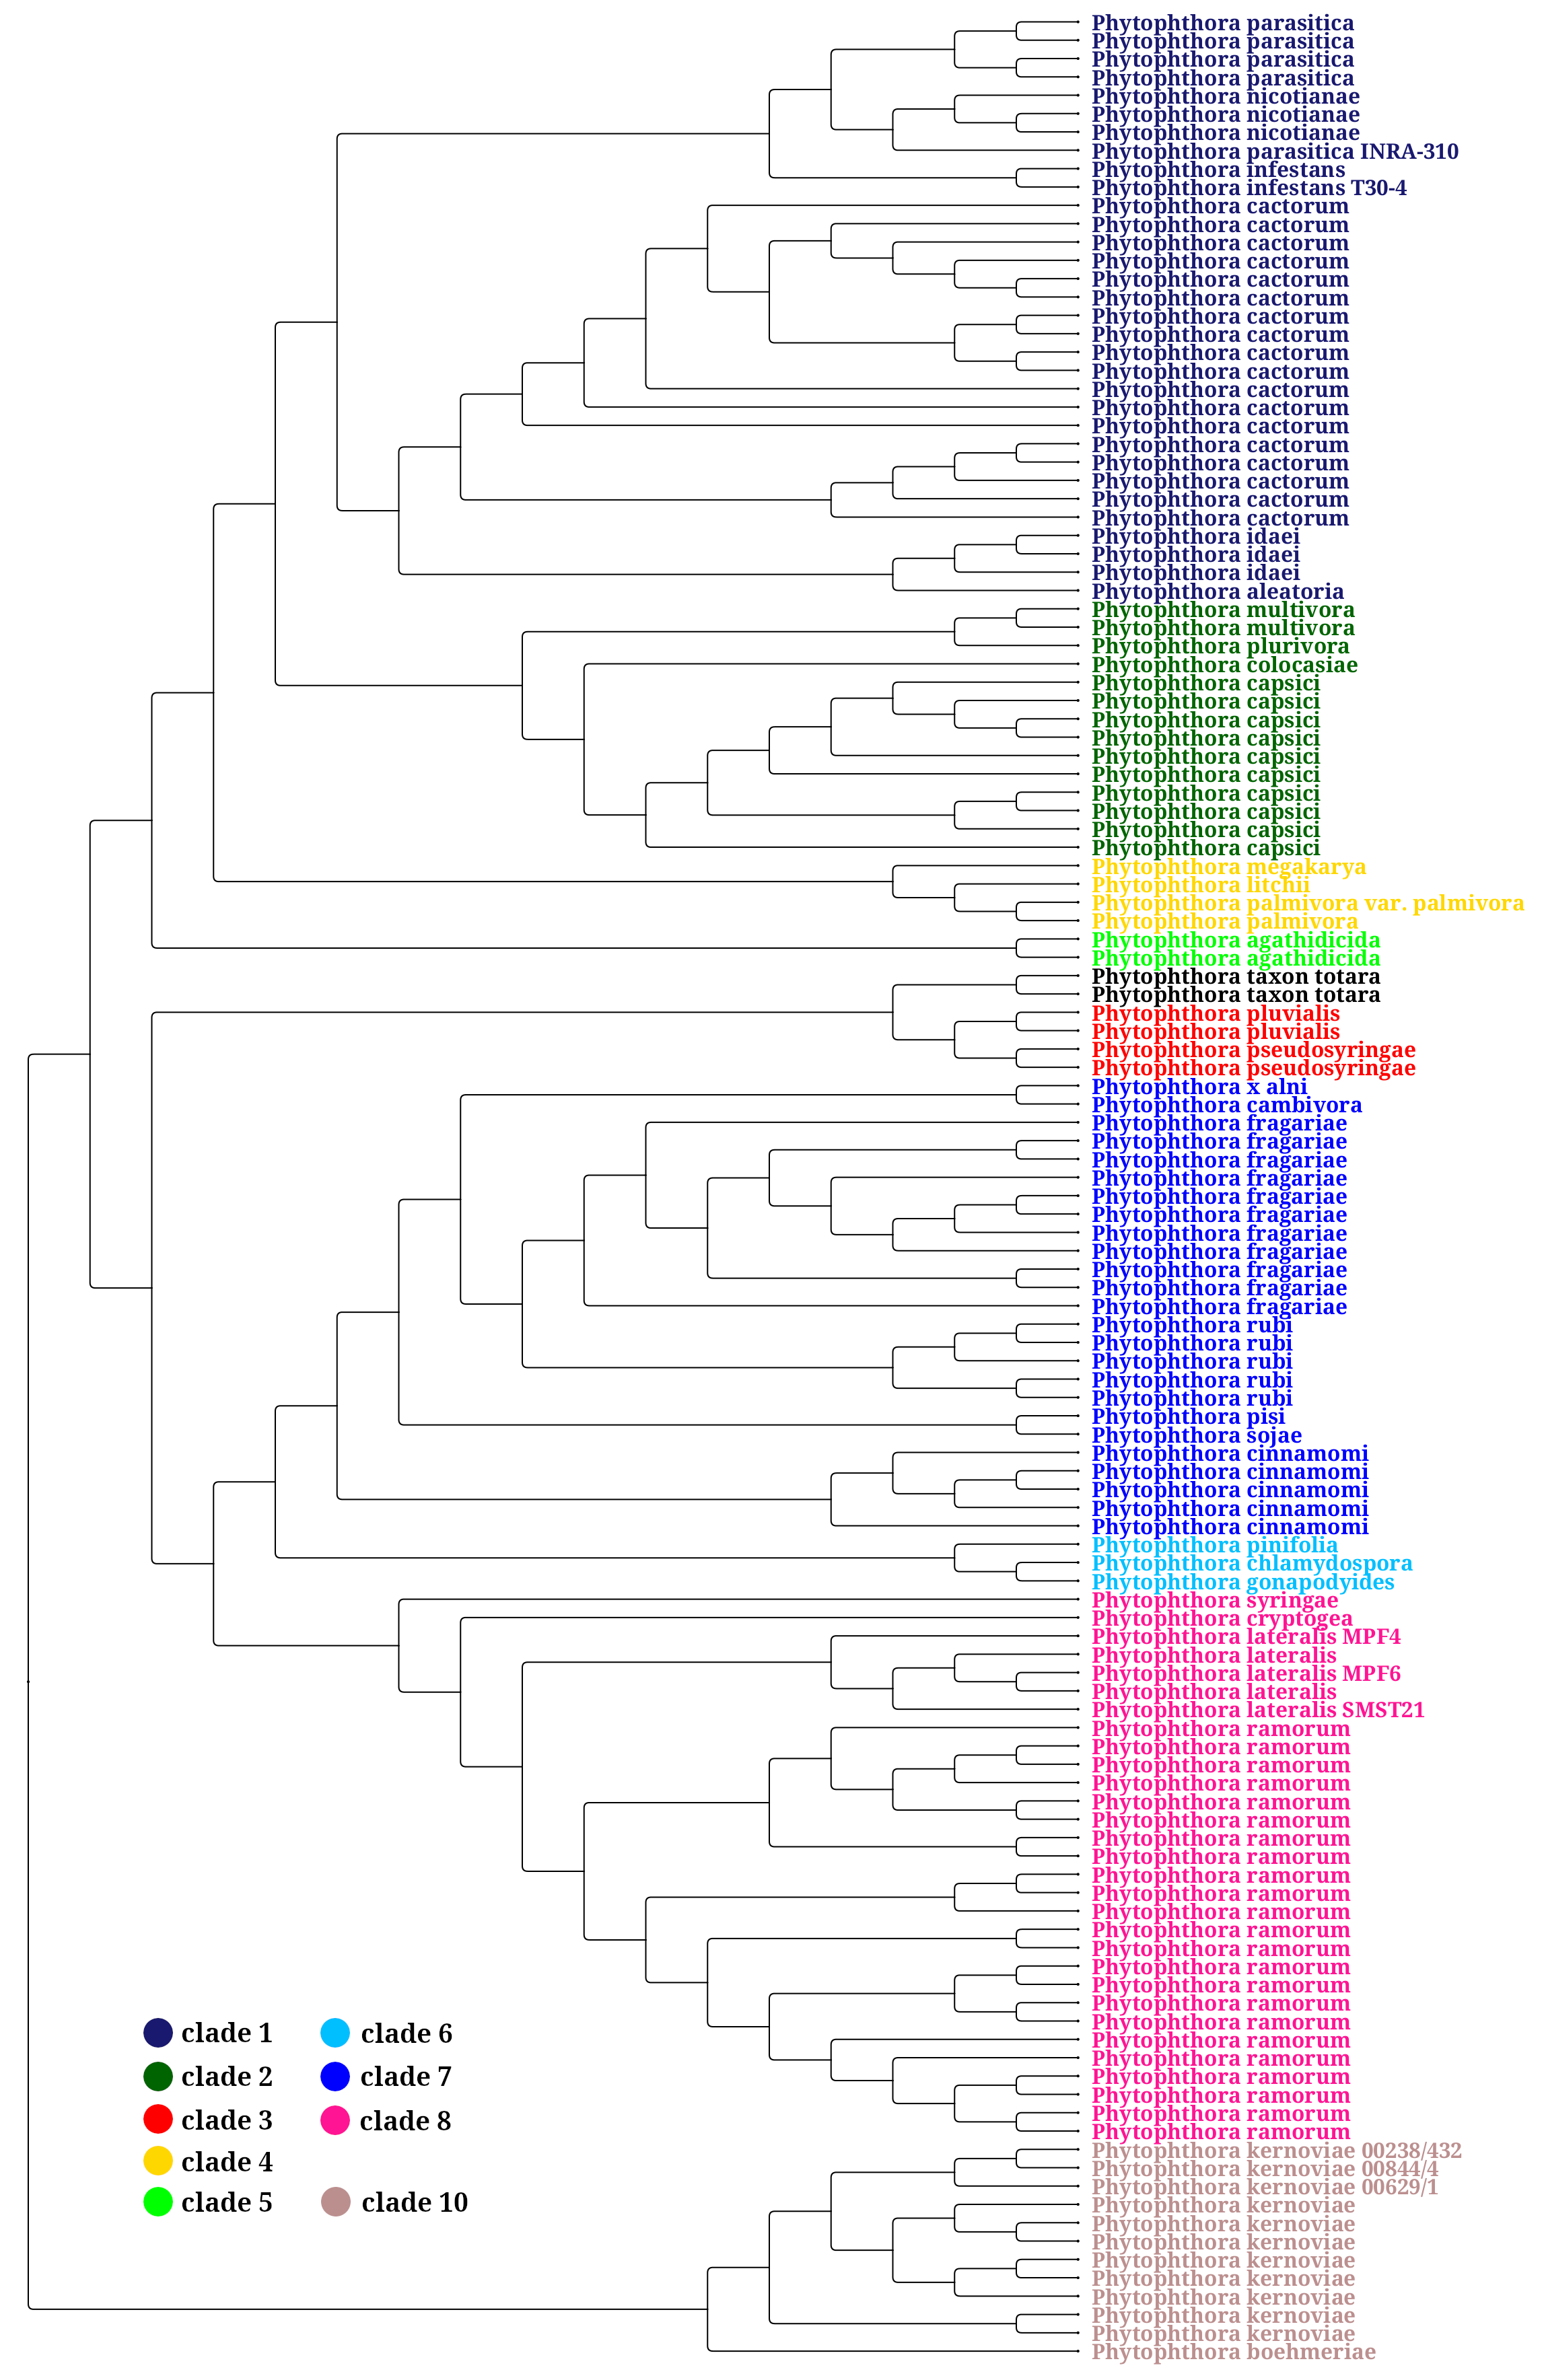
\includegraphics[width=1.0\textwidth]{figures/fmhdist_mandal_tree_k21_s2000.png}
  \caption{Phylogenetic tree based on distances of datasetA calculated with
  \texttt{fmhdist}. Taxa are colored according to clade membership
  \cite{abadPhytophthoraTaxonomicPhylogenetic2023a}. The tree is rooted with
  clade 10 as outgroup.}
  \label{fig:mandalFmhdistTree}
\end{figure}

\todo{maybe reference consensus network here?}

\subsection*{Outlines}
The phylogenetic outline that was calculated using the re-computed Mash
distances for dataset A is shown in Figure~\ref{fig:mandalMashOutline}. Similar
to the trees, clusters are well defined and in line with literature
\cite{abadPhytophthoraTaxonomicPhylogenetic2023a,yangExpandedPhylogenyGenus2017}.
The outline also visualizes the subclades rather well.

\begin{figure}
  \centering
  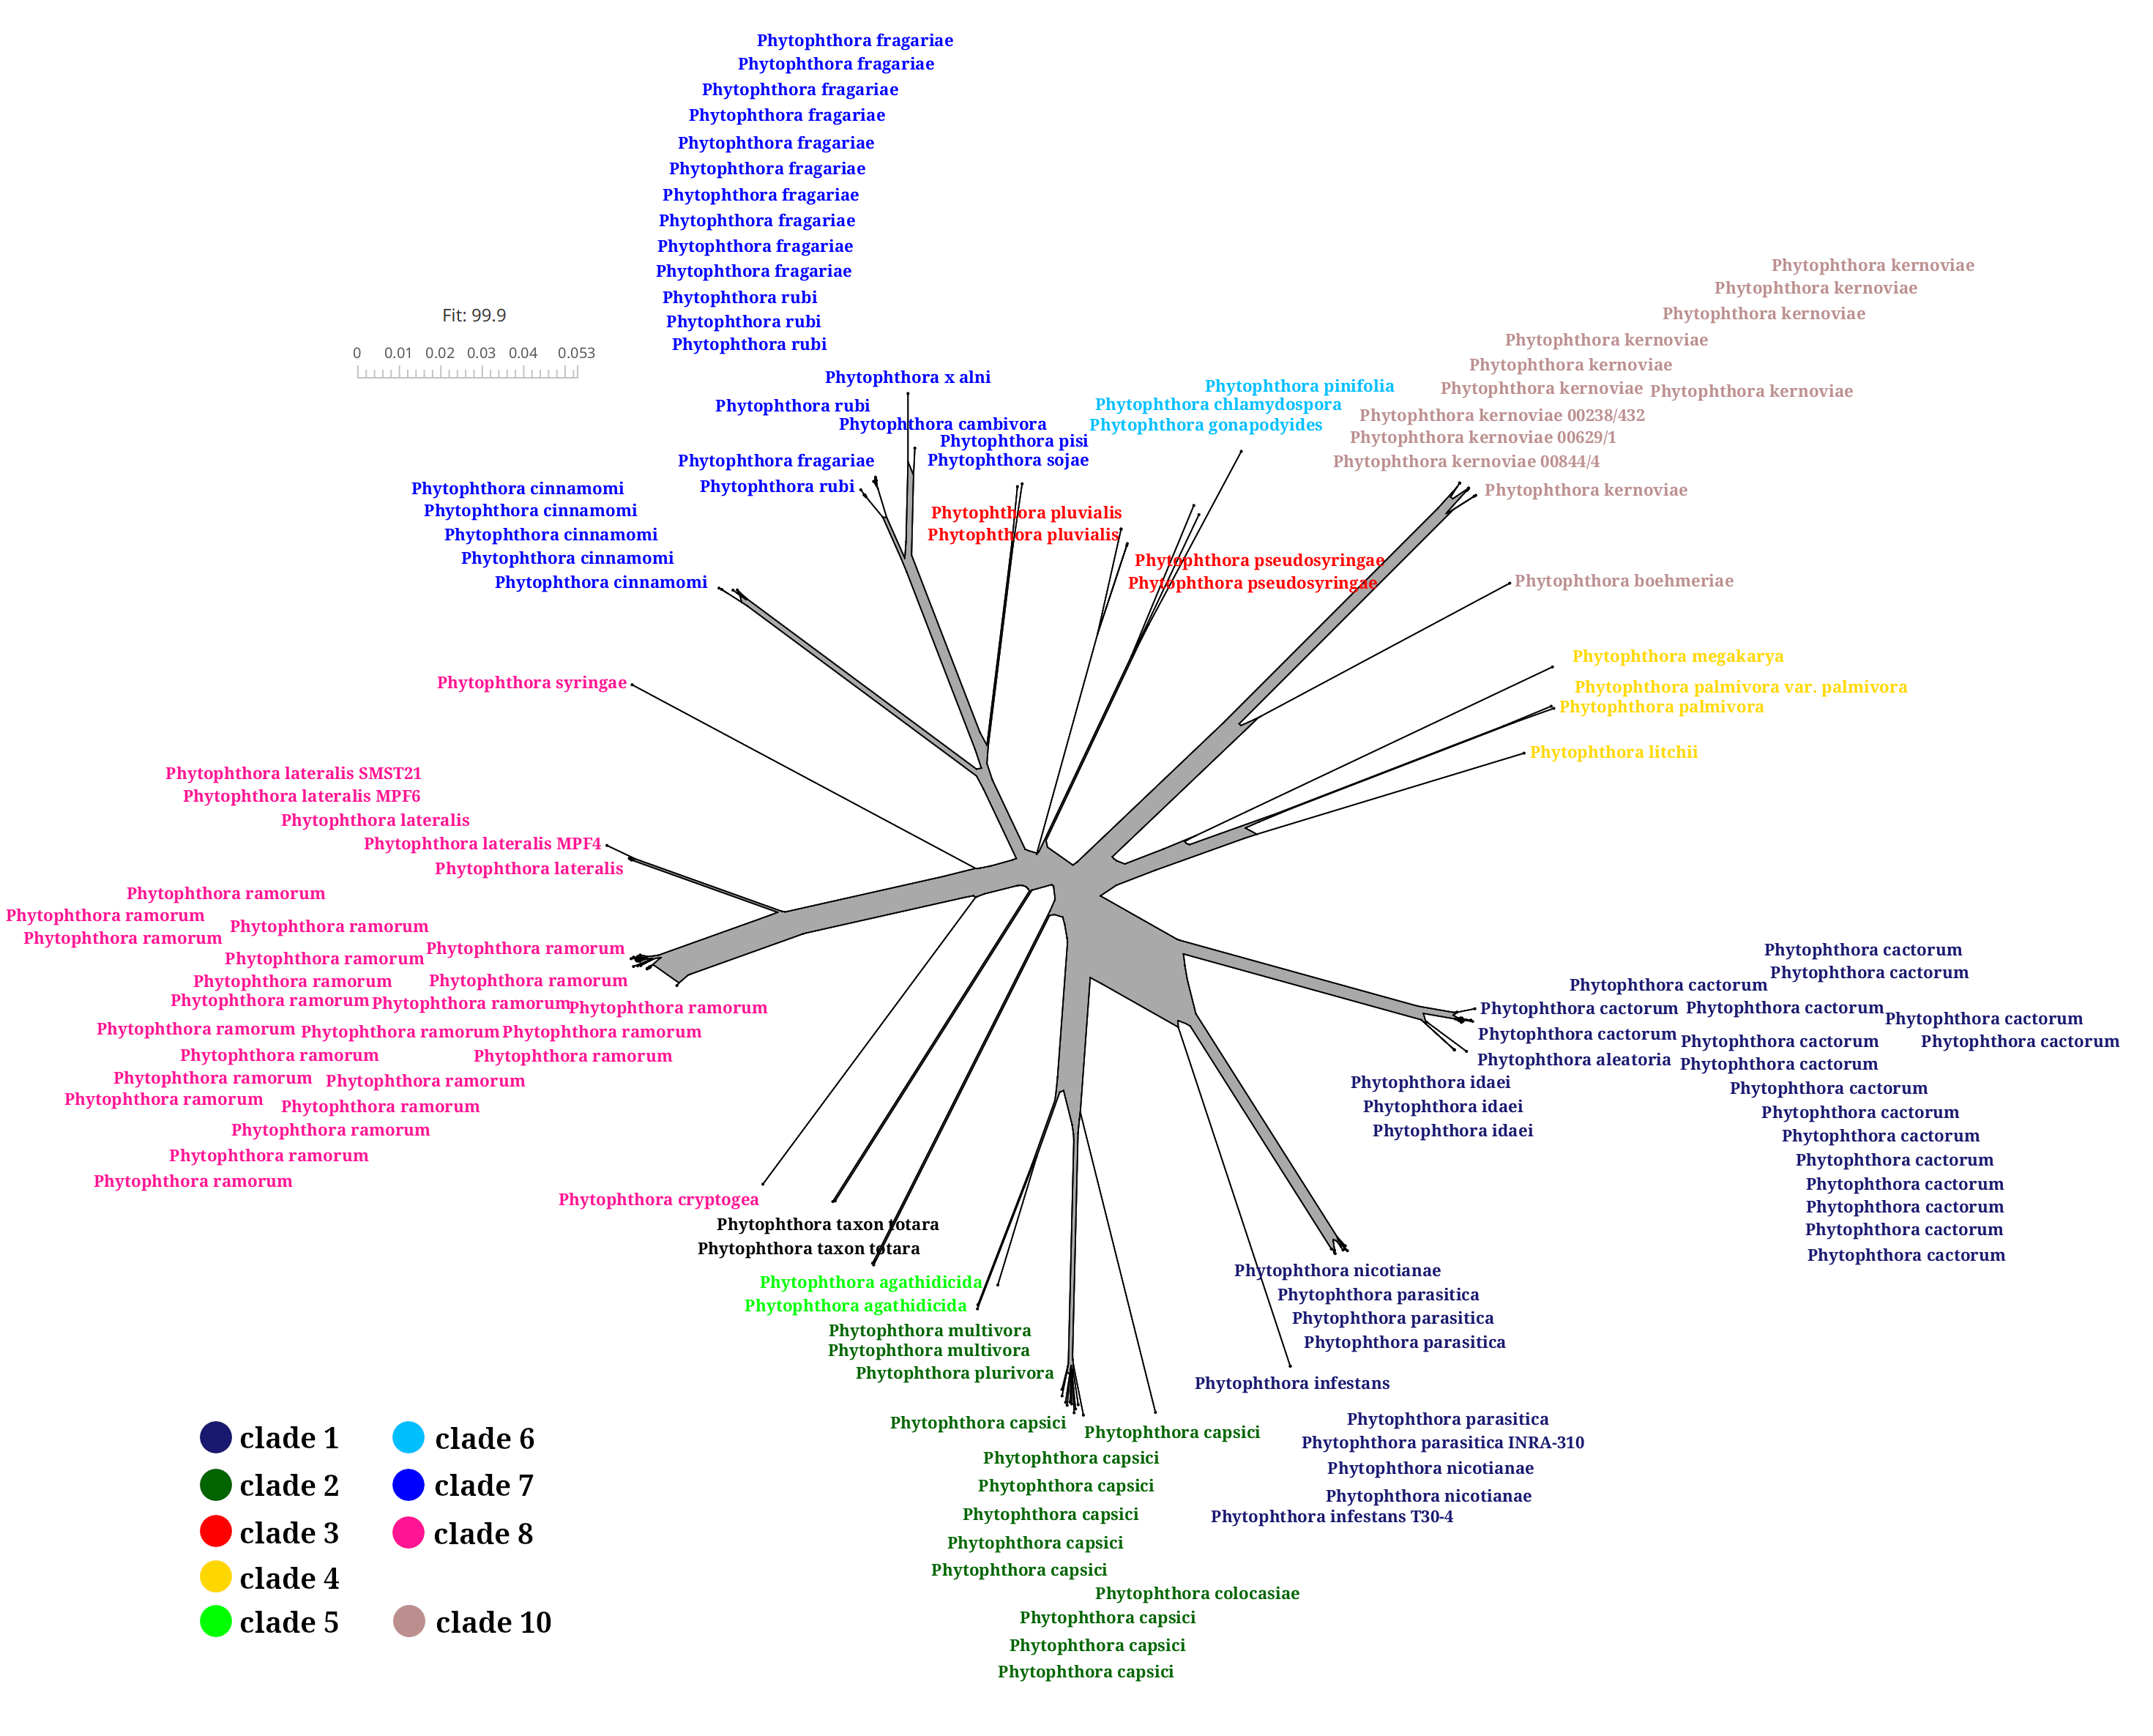
\includegraphics[width=1.0\textwidth]{figures/mashtree_mandal_outline_k21_s2000.png}
  \caption{Phylogenetic outline based on distances of dataset A calculated with
  \texttt{mashtree}
  \cite{ondovMashFastGenome2016,katzMashtreeRapidComparison2019}. Taxa are
  colored according to clade membership
  \cite{abadPhytophthoraTaxonomicPhylogenetic2023a}.}
  \label{fig:mandalMashOutline}
\end{figure}

The phyloegenetic outline that was calculated using the FracMinHash distance for
dataset A is depicted in Figure~\ref{fig:mandalFmhdistTree}. Again, clusters are
well defined and in line with literature, the same holds for the subclades
\cite{abadPhytophthoraTaxonomicPhylogenetic2023a,yangExpandedPhylogenyGenus2017}.

\begin{figure}
  \centering
  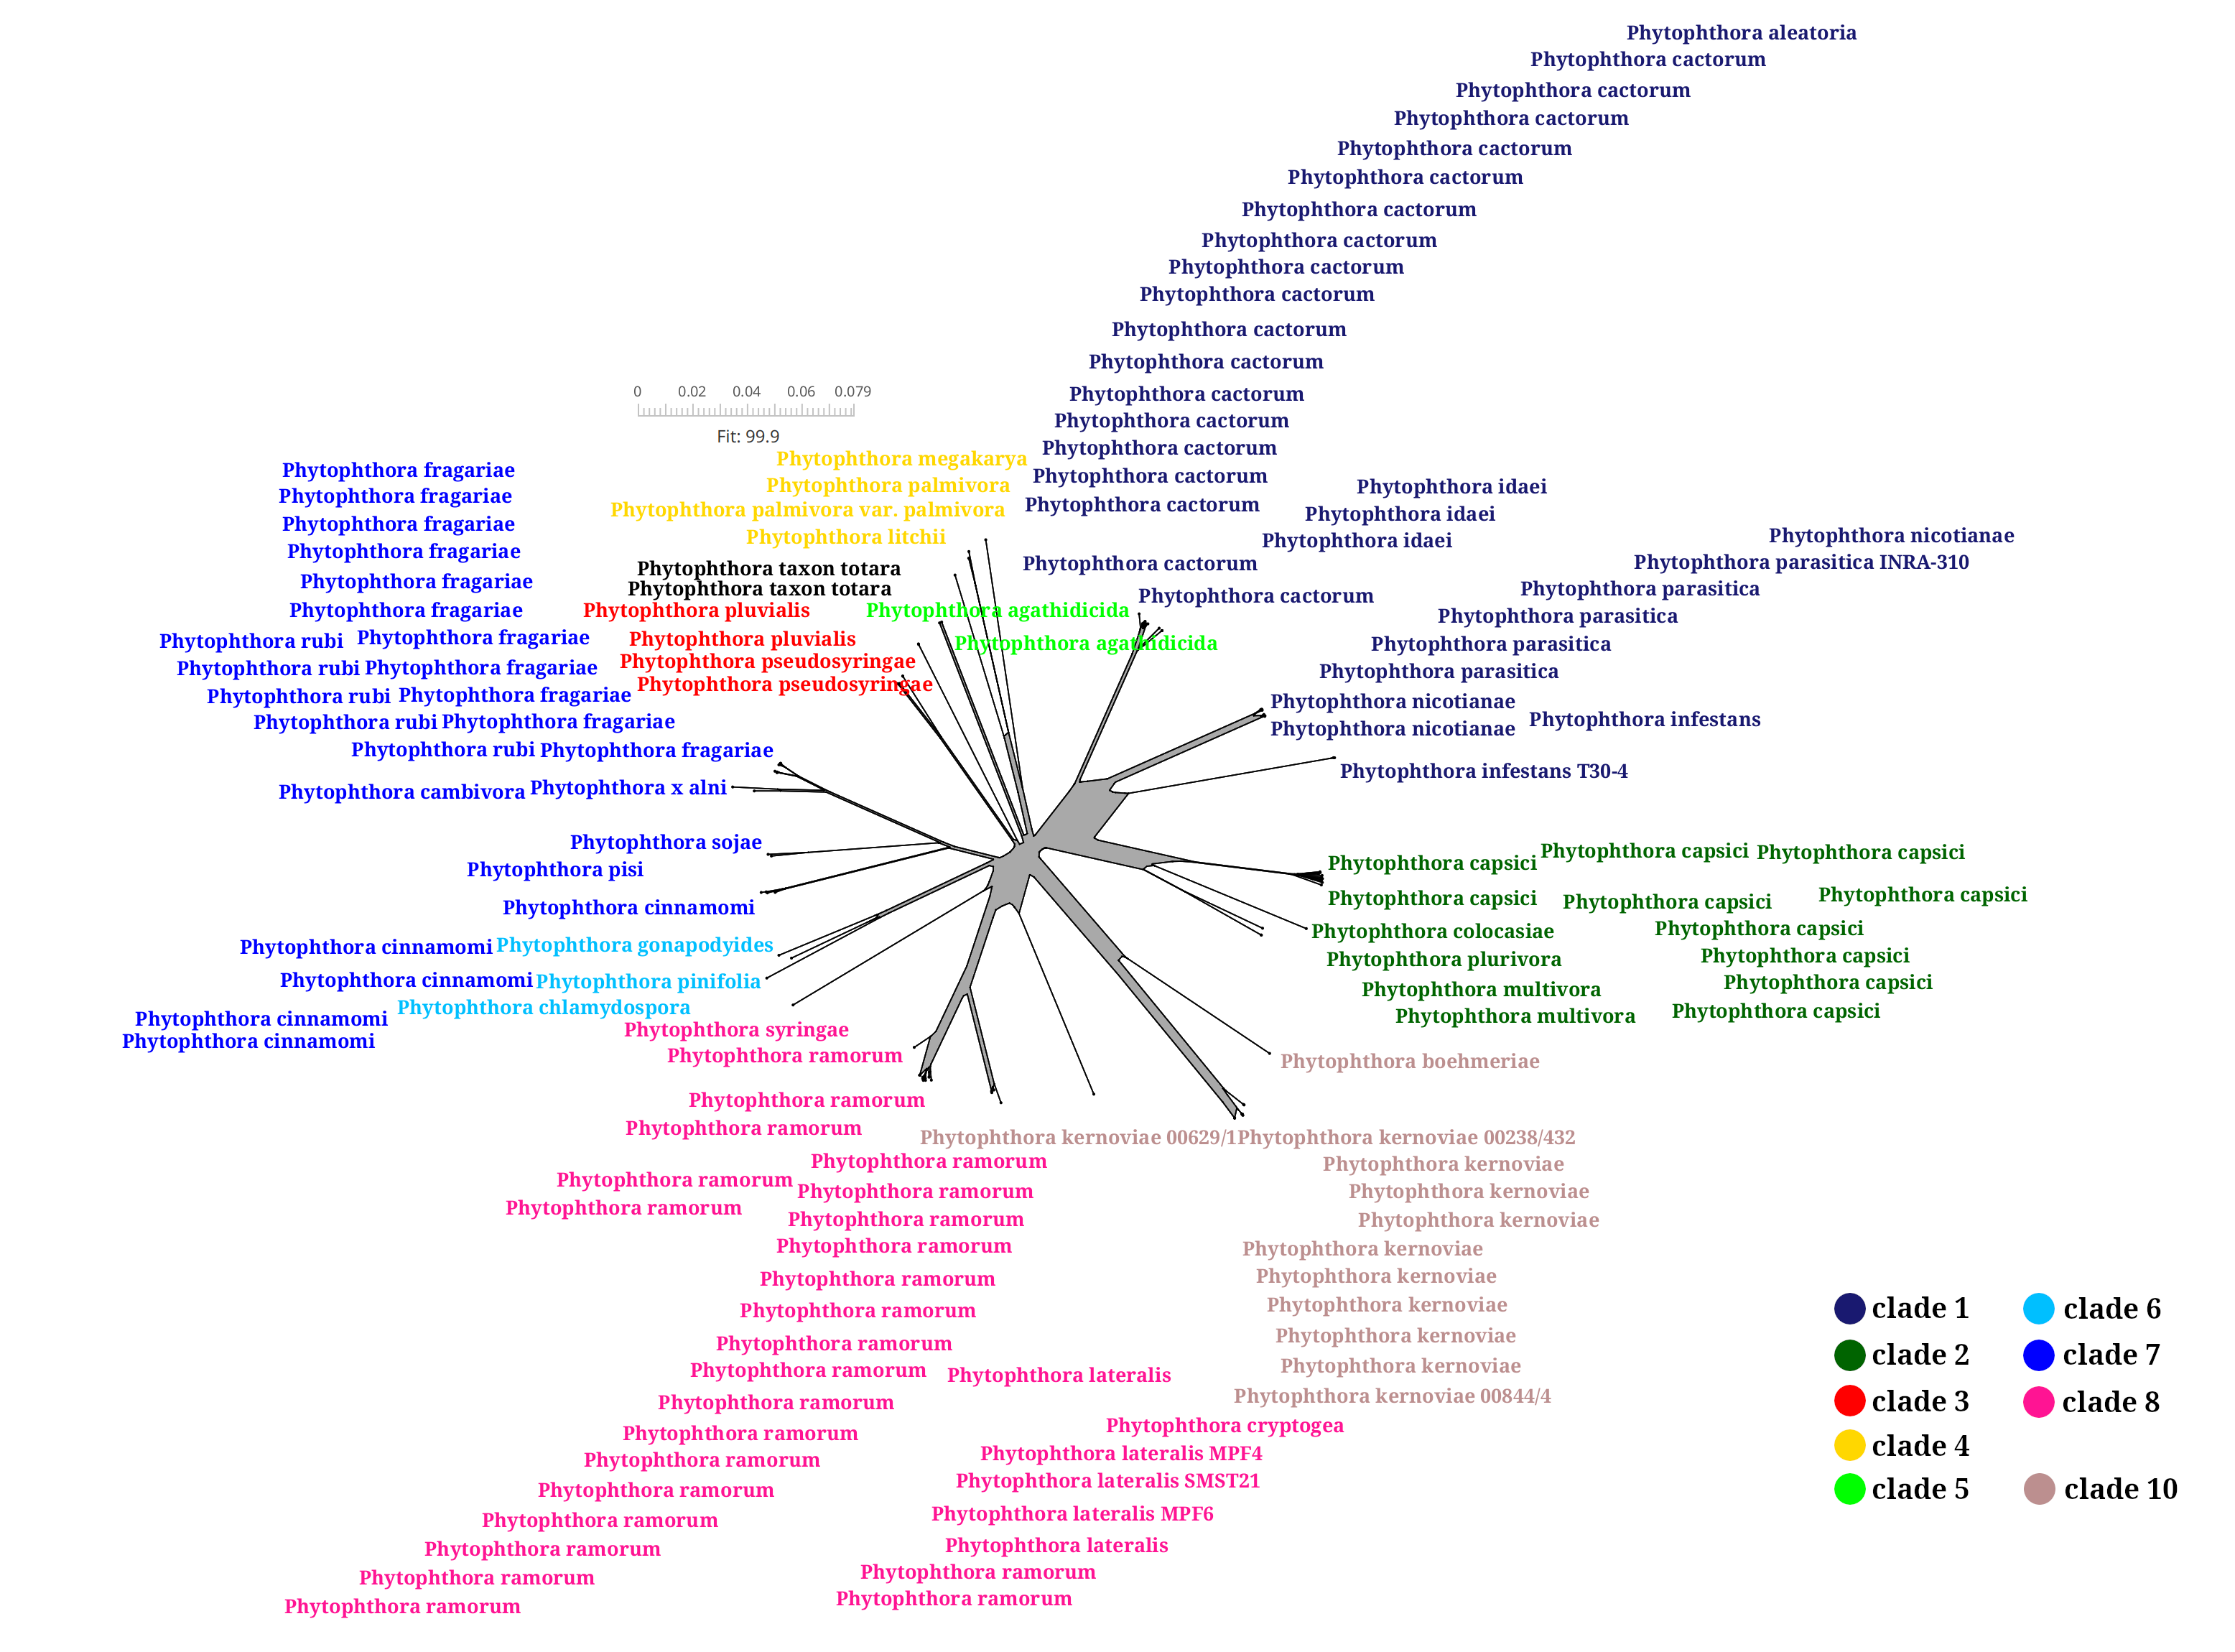
\includegraphics[width=1.0\textwidth]{figures/fmhdist_mandal_outline_k21_s2000.png}
  \caption{Phylogenetic outline based on distances of dataset A calculated with
  \texttt{fmhdist}. Taxa are colored according to clade membership
  \cite{abadPhytophthoraTaxonomicPhylogenetic2023a}.}
  \label{fig:mandalFmhdistOutline}
\end{figure}

Comparing the outlines and the underlying splits, one noteable difference is the
relationship betwen clades 8 and 10. The \texttt{fmhdist} distances provide a
split $S= \{1, 2, 3, 4, 5\} | \{6, 7, 8, 10\}$ and $S= \{1, 2, 3, 4, 5, 6, 7\} |
\{8, 10\}$. Although those clade clusters are in line with literature
\cite{yangExpandedPhylogenyGenus2017,abadPhytophthoraTaxonomicPhylogenetic2023a},
they are not present when using the \texttt{mashtree} distances.


\section{Split differences are measurable}
As seen in Table~\ref{ta:splitDifferences}, the splits generated from the
\texttt{mashtree} distances differ from the splits generated by
\texttt{fmhdist}, i.e. there are splits in the former that are not in the latter
and vice versa. Compared to the difference between the three different distance
metrics implemented in \texttt{fmhdist}, we can observe that the number of
split differences is much smaller and thus the total weight associated with
those differences. The Robinson-Foulds distance $D_{RF}$ is very similar in all
three comparisons.

\begin{table}[]
  \centering
  \begin{tabular}{@{}lrrr@{}}
    \toprule
    &  \textbf{I} & \textbf{II} & \textbf{III} \\
    \midrule
  $\sum_{s \in \Sigma_A}{\omega(s)}$           & 1.3064                     & 1.3064                              & 1.3064                         \\
  $\sum_{s \in \Sigma_B}{\omega(s)}$           & 1.4321                     & 1.2990                              & 1.4339                         \\
  $\sum_{s \in \Sigma_A / \Sigma_B}{\omega(s)}$ & 0.1059                    & 0.0174                              & 0.0299                      \\
  $\sum_{s \in \Sigma_B / \Sigma_A}{\omega(s)}$ & 0.1061                    & 0.0142                             & 0.0335                       \\
  $|\Sigma_A / \Sigma_B|$                       & 103                       & 31                                 & 54                                        \\
  $|\Sigma_B / \Sigma_A|$                       & 75                        & 27                                 & 48                                        \\
  $D_{RF}(\Sigma_A, \Sigma_B)$                 & 149.0                       & 161.0                                & 160.5         \\
  \bottomrule                           
  \end{tabular}
  \caption{Comparison of different sets of splits based on different distance
  calculations of dataset A. \textbf{I} is the comparison of \texttt{fmhdist}
  against \texttt{mashtreee}. \textbf{II} is the comparison of \texttt{fmhdist}
  against \texttt{fmhdist containment}. \textbf{III} is the comparison of
  \texttt{fmhdist} against \texttt{fmhdist mash}.}
  \label{ta:splitDifferences}
\end{table}


\section{Impact of parameter choices}
\subsection*{Impact of the choice of $k$ and $s$}
At the typical $k$-mer size of $k=21$
\cite{mandalComparativeGenomeAnalysis2022,ondovMashFastGenome2016,irberLightweightCompositionalAnalysis2022},
the method performs well as described above. Using $k \in \{19, 20, 22, 25\}$
does not change the produced outline substantially. This is also backed by the
calculated sum of split weights and the differences therein. Comparing $k=21$
with $k=25$ indicates a very small difference in the total weight ($1.3064$ vs
$1.2413$), a difference that is smaller than comparing Mash and FracMinHash.
Extreme values, such as $k=10$ break the clusters such that species are not
clustered accoding to clade membership anymore. Using such a small $k$ leads to
a very low total weight of splits ($0.3374$) and in general unusual outlines.

Different values of $s$ change the sketch size. Using $s=2000$, the the sketch
sizes range from $17397$ to $66726$ with a median at $24906$. Using $s=4000$,
the sketch sizes range from $8738$ to $33504$ with a median at $12423$. The
sketch sizes are clearly halved which is to be expected when doubling $s$.

The impact of changing $s$ in the given range is small in terms of splits and
outlines. Changing $s$ rotates or mirrors some relationships, introduces splits
and removes others, but all of those differences have minor impact on
interpreting the generated outline. This is also indicated by the differences in
split weight, the total weight of splits for the four different variants of $s$
is in the interval $[1.3064, 1.3165]$. The weight of split differences is the
range $[0.0419, 0.0805]$.

\subsection*{Impact of the choice of hash function}
While all hash functions are capable of hashing tens of millions keys of size
$21$ per second, the runtime varies a lot when looked at closer
(Table~\ref{ta:hashbenchmark}). The best runtime for keys of size $21$ was
achieved with the two variants of FarmHash, followed by WyHash and CityHash. The
hash function used by \texttt{mash} and \texttt{sourmash}, MurMur3
\cite{ondovMashFastGenome2016,irberLightweightCompositionalAnalysis2022}, only
achieves medium speed in comparison to the other hash functions.  

\begin{table}[]
  \centering
  \begin{tabular}{@{}lr@{}}
  \toprule
  \textbf{Hash Function }& \textbf{Throughput (ops/s)}                      \\
  \midrule
  CityHash      & 53502048.778 ± 4483465.863   \\
  FarmHash 1.0  & 55008714.492 ± 2363256.004   \\
  FarmHash 1.1  & 54678293.943 ±  482133.235   \\
  MetroHash     & 51132334.855 ±  307903.868   \\
  MurMur 3      & 36500708.446 ±  497774.958   \\
  WyHash        & 54259034.831 ± 1327599.078   \\
  XX128         & 22684338.104 ±   98278.977   \\
  XX3           & 27170615.109 ±  220725.087   \\
  XX64          & 44799765.447 ± 1091771.572  \\
  \bottomrule
  \end{tabular}
  \caption{Results of the hash function benchmark for keys of size $21$.}
  \label{ta:hashbenchmark}
  \end{table}


\section{Sketches of mtDNA are very small}
Outlines and trees generated from the FracMinHash distances for dataset B with
$s=1000$ are not usable. Most of the distances are 0, thus edge lengths are too
short to separate taxa in any meaningful way. The smallest sketch has $29$
$k$-mers, the largest $54$. The same behaviour can be observed when sketching
viral genomes stored in NCBI. Using smaller values for $s$ creates clusters that
resemble the clade membership well
\cite{abadPhytophthoraTaxonomicPhylogenetic2023a,yangExpandedPhylogenyGenus2017}.
The outlines from dataset B with $s=100$ are depicted in
Figure~\ref{fig:winkworthTree}. Here, sketch sizes range from $333$ to $454$.
Comparing the trees and outlines for $s=1$ values to published phylogenies
\cite{abadPhytophthoraTaxonomicPhylogenetic2023a,yangExpandedPhylogenyGenus2017},
we can observe that several relationships between clade are not depicted, e.g.
the clades 1, 2 and 4 or the clades 8 and 10 can only be clustered when adding
more clades.


The tree published in \cite{winkworthComparativeAnalysesComplete2022} has the
following topology:

\texttt{((((((((((1, 16), 4), 3), (2, (5, 12)), 15), 6),
7), 8), (9, 10), \textit{Nothophytophthora sp.}), \textit{Phytopythium vexans}),
\textit{Phytium ultimum})}

The FracMinHash tree as depicted in Figure~\ref{fig:winkworthTree} has the topology

\texttt{(((((((((((5, 12), 15b), 1), (3, 4)), (8, (6, (7, 2)))), (9, 10)), 16),
15a), \textit{Nothophytophthora sp.}), \textit{Phytopythium
vexans}), \textit{Phytium ultimum})}


There are so many differences in the trees that it is easier to list shared
aspects. Noteably, the clustering of clades 5 and 12, and 9 and 10 as well as
the placement of the outgroups\textit{Phytium ultimum}, \textit{Phytopythium
vexans} and \textit{Nothophytophthora sp.} are shared between the two trees.

\begin{figure}
  \centering
  \includegraphics[width=1.0\textwidth]{figures/fmhdist_winkworth_tree_k21_s100.png}
  \caption{Phylogenetic tree based on distances calculated with \texttt{fmhdist}
  for dataset B using $k=21$ and $s=100$. Taxa are colored according to clade
  membership
  \cite{abadPhytophthoraTaxonomicPhylogenetic2023a,winkworthComparativeAnalysesComplete2022}.
  The tree is rooted with \textit{Phytium ultimum} as outgroup.}
  \label{fig:winkworthTree}
\end{figure}

\section{FracMinHash estimates distances for distantly related genomes}
The different outlines based on the \texttt{mashtree} and \texttt{fmhdist}
($s=2000$) distances of dataset C, respectively, are depicted in
Figure~/ref{fig:avocadoOutlineComparison}. Of interest is the placement of the
query genomes, the bacterial queries are very clearly separated from the all
\textit{Phytophthora} reference genomes in both outlines. This is not true for
the two fungal queries, they are placed in between the \textit{Phytophthora}
reference genomes in the \texttt{fmhdist} variant but also as outliers in the
\texttt{mashtree} variant.

\begin{figure}
  \centering
  \begin{subfigure}{0.49\textwidth}
    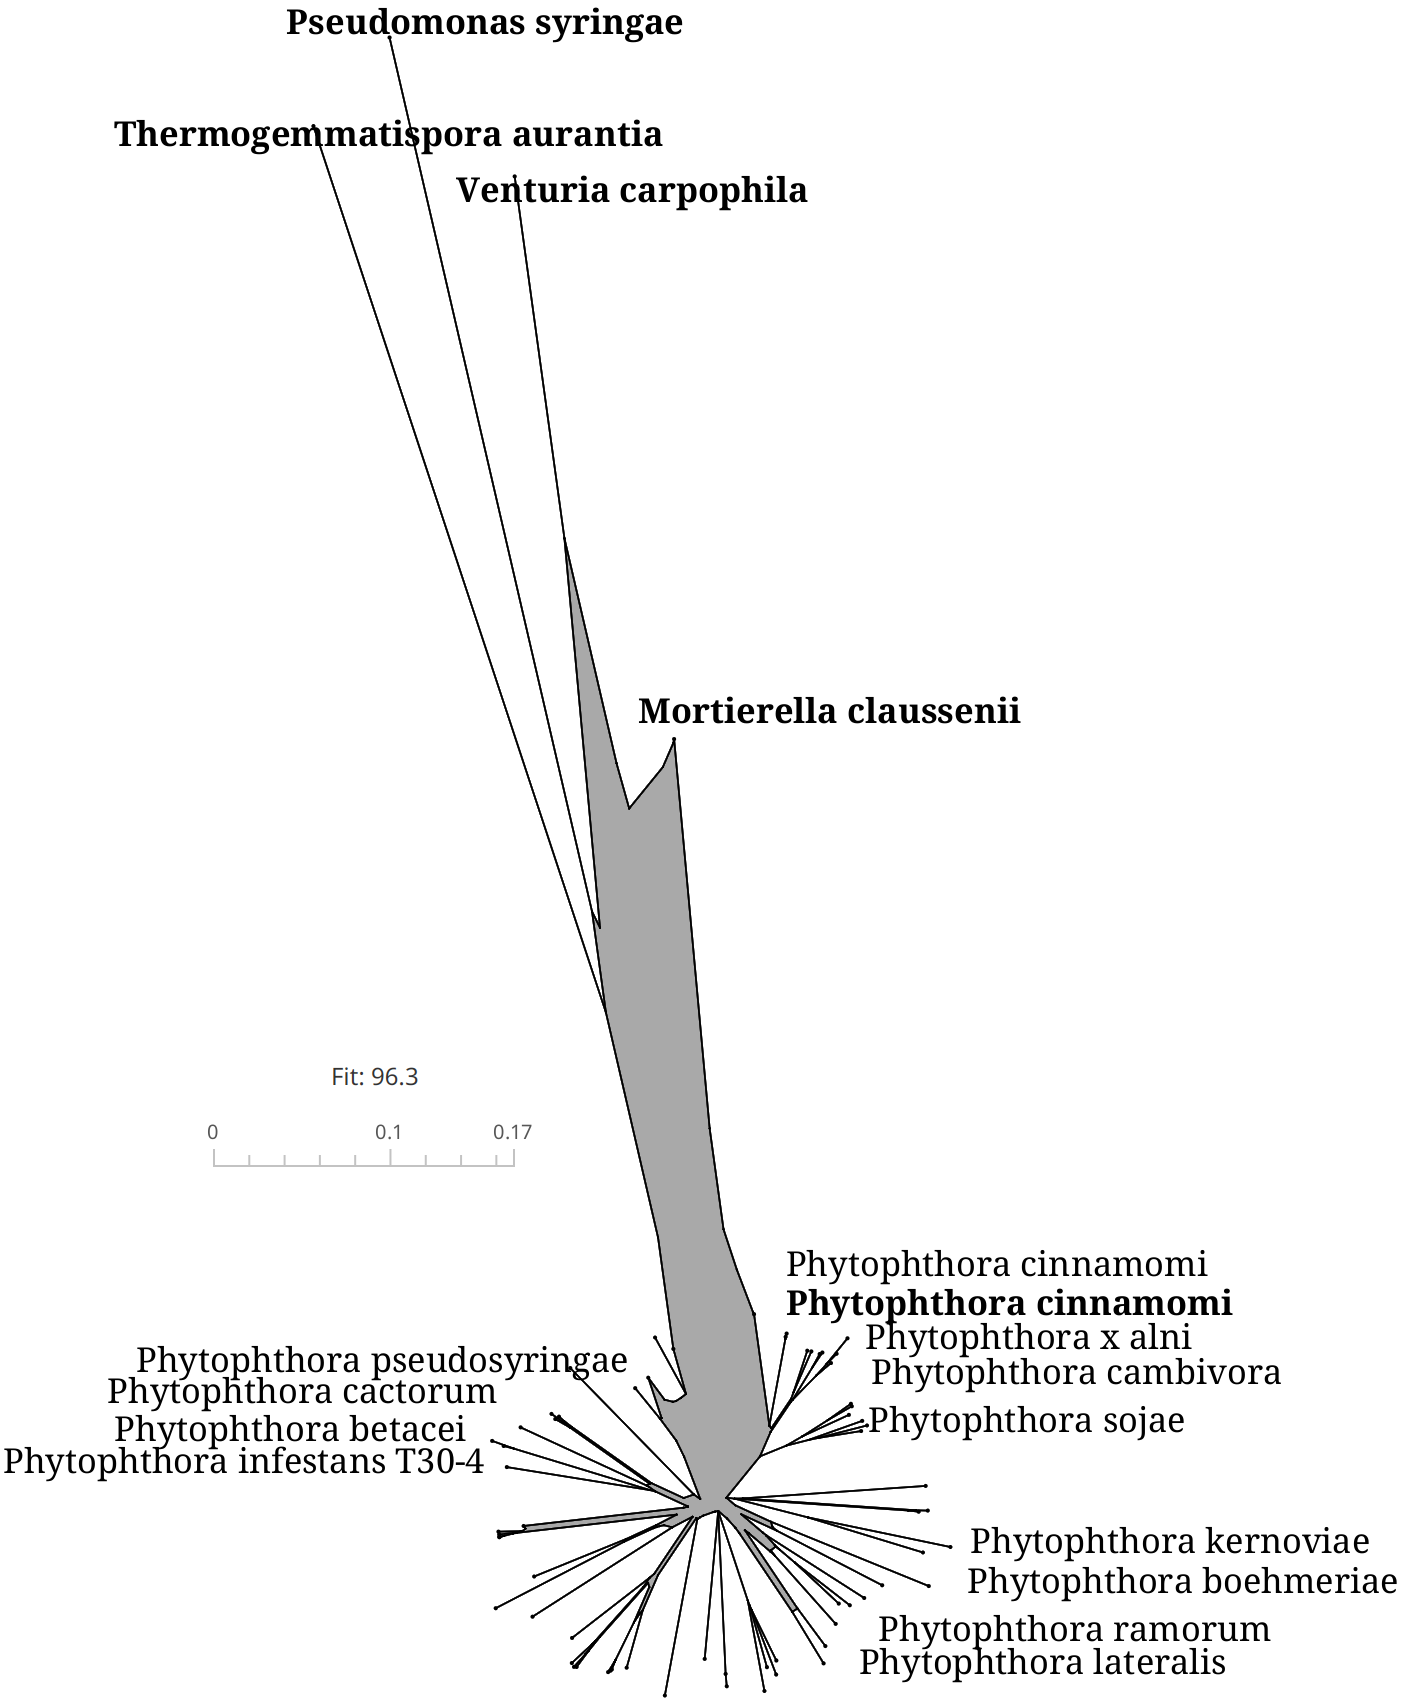
\includegraphics[width=1.0\textwidth]{figures/mashtree_avocado4-1_k21_s2000.png}
  \end{subfigure}
  \begin{subfigure}{0.49\textwidth}
    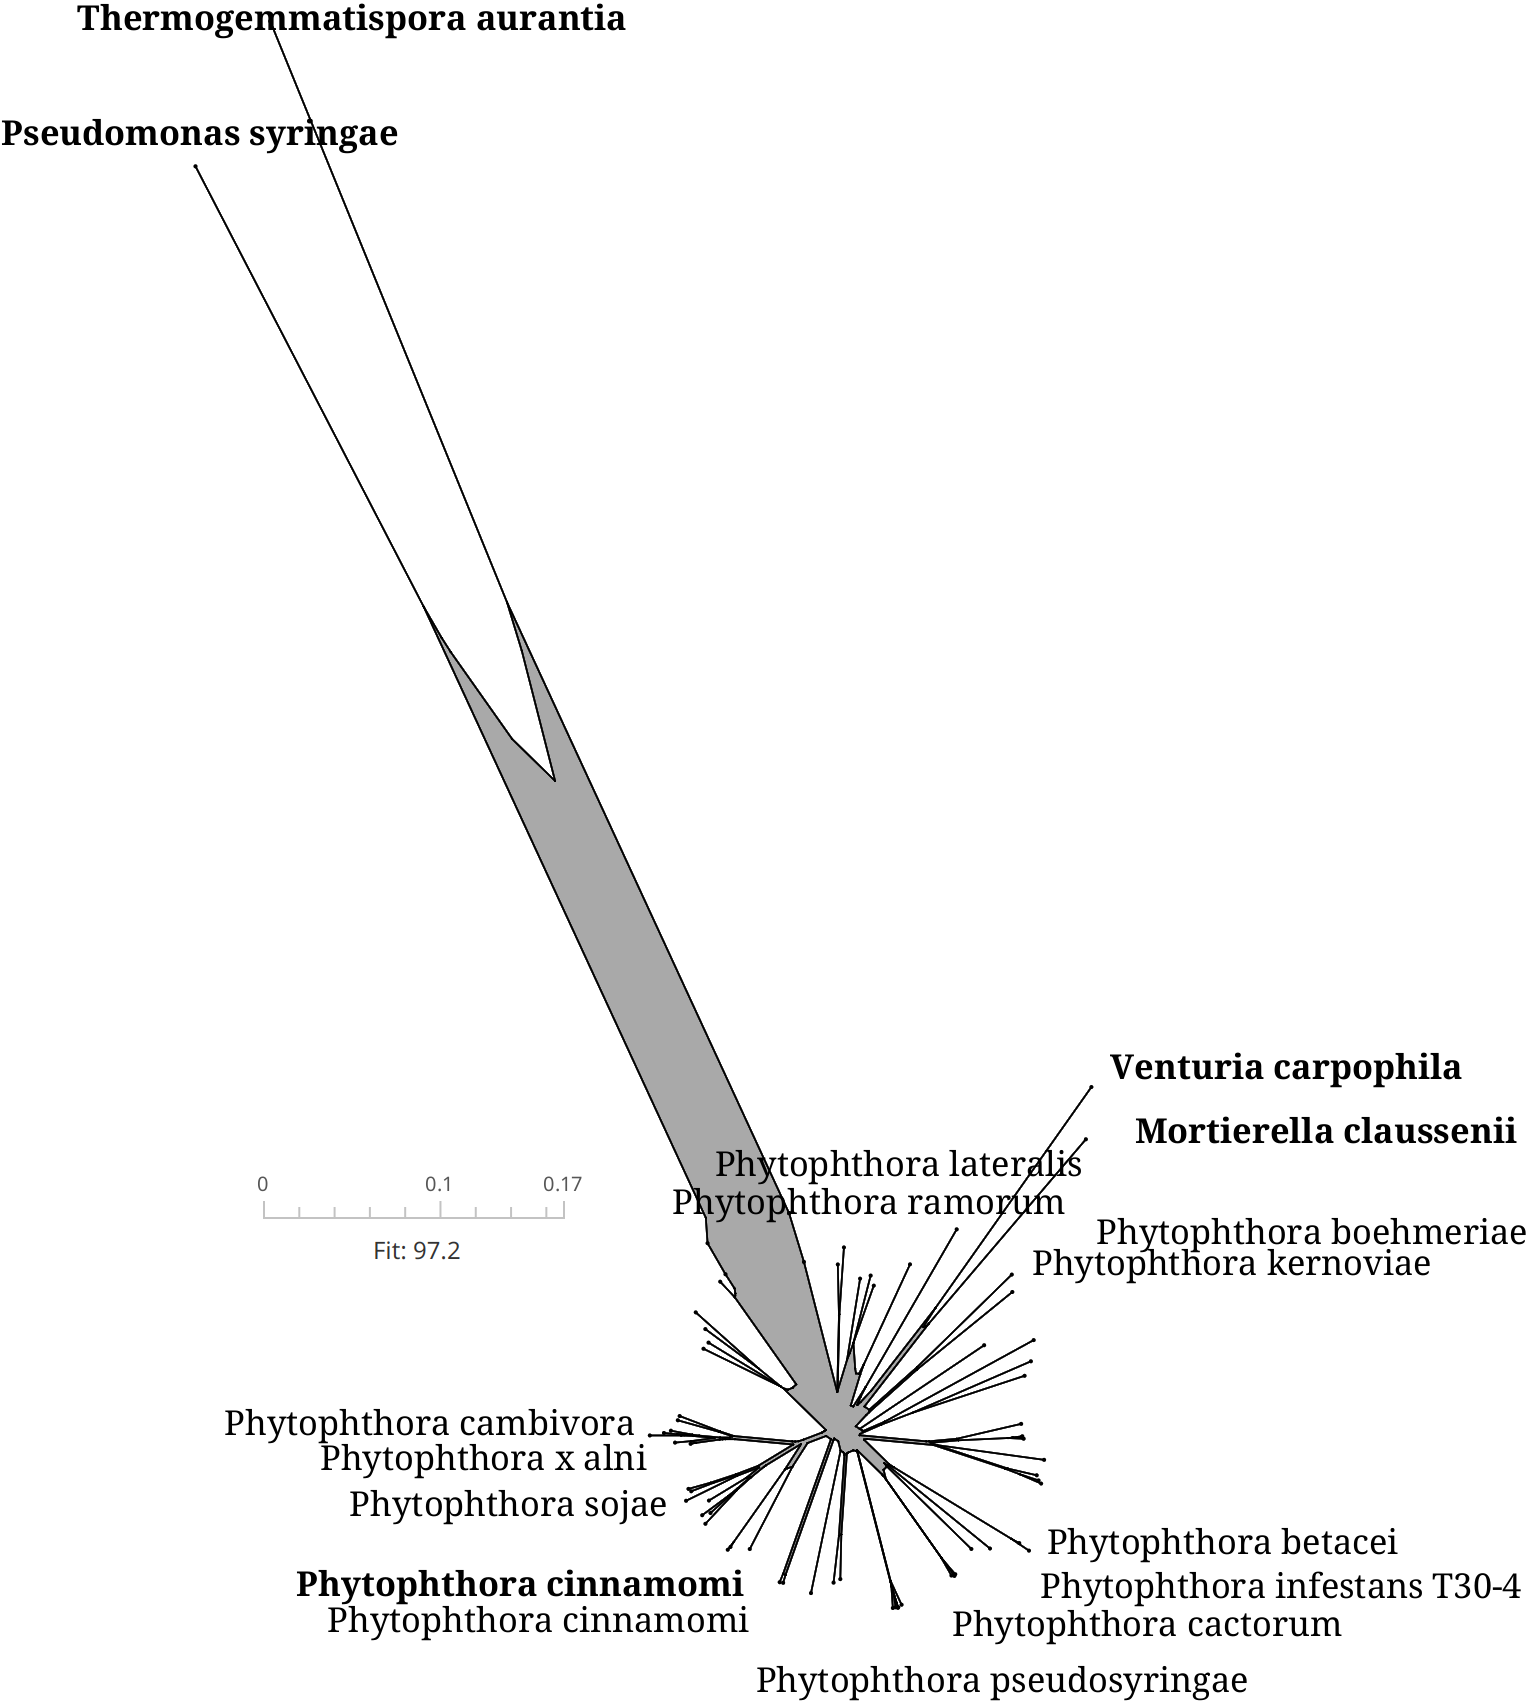
\includegraphics[width=1.0\textwidth]{figures/fmhdist_avocado4-1_k21_s2000.png}
  \end{subfigure}
  \caption{caption}
  \label{fig:avocadoOutlineComparison}
\end{figure}

This behaviour can obviously also be observed when comparing the distances of
the five queries and the \textit{Phytophthora infestans} reference directly
(Table~\ref{ta:avocadoDistance}). All distances involving the bacterial queries
are $1.0$.

The mash distance for \textit{Venturia carpophila} is $1.0$ for the comparison
the bacterial queries and \textit{Phytophthora infestans} and
\textit{Phytophthora cinnamomi} and $0.3726$ for the comparison with the other
fungal query, \textit{Mortierella claussenii}. This query, in turn, does have
low distances of $0.3290$ and $0.4056$ to \textit{Phytophthora cinnamomi} and
\textit{Phytophthora infestans}, respectively.

For FracMinHash, we can see that both fungal queries have a distance below 1 to
the two \textit{Phytophthora} genomes.


% Please add the following required packages to your document preamble:
% \usepackage{booktabs}
\begin{table}[]
  \centering
  \begin{tabular}{@{}llrrrrrr@{}}
  \toprule
              &                      & \textbf{F1} & \textbf{F2} & \textbf{B1} & \textbf{B2} & \textbf{P1} & \textbf{P2} \\ \midrule
  \textbf{F1} & \textbf{Mash}        & 0.0000      & 0.3726      & 1.0000      & 1.0000      & 0.3290      & 0.4056      \\
  \textbf{}   & \textbf{FracMinHash} & 0.0000      & 0.3024      & 1.0000      & 1.0000      & 0.3010      & 0.3101      \\ \midrule
  \textbf{F2} & \textbf{Mash}        & 0.3726      & 0.0000      & 1.0000      & 1.0000      & 1.0000      & 1.0000      \\
  \textbf{}   & \textbf{FracMinHash} & 0.3024      & 0.0000      & 1.0000      & 1.0000      & 0.3278      & 0.3338      \\ \midrule
  \textbf{B1} & \textbf{Mash}        & 1.0000      & 1.0000      & 0.0000      & 1.0000      & 1.0000      & 1.0000      \\
  \textbf{}   & \textbf{FracMinHash} & 1.0000      & 1.0000      & 0.0000      & 1.0000      & 1.0000      & 1.0000      \\ \midrule
  \textbf{B2} & \textbf{Mash}        & 1.0000      & 1.0000      & 1.0000      & 0.0000      & 1.0000      & 1.0000      \\
  \textbf{}   & \textbf{FracMinHash} & 1.0000      & 1.0000      & 1.0000      & 0.0000      & 1.0000      & 1.0000      \\ \midrule
  \textbf{P1} & \textbf{Mash}        & 0.3290      & 1.0000      & 1.0000      & 1.0000      & 0.0000      & 0.2470      \\
  \textbf{}   & \textbf{FracMinHash} & 0.3010      & 0.3278      & 1.0000      & 1.0000      & 0.0000      & 0.2252      \\ \midrule
  \textbf{P2} & \textbf{Mash}        & 0.4056      & 1.0000      & 1.0000      & 1.0000      & 0.2470      & 0.0000      \\
  \textbf{}   & \textbf{FracMinHash} & 0.3101      & 0.3338      & 1.0000      & 1.0000      & 0.2252      & 0.0000      \\ \bottomrule
  \end{tabular}
  \caption{Distance estimation calculated with \texttt{mashtree} with default
  settings and \texttt{fmhdist} with $k=21$, $s=2000$, FarmHash and random seed
  $rs=42$ for \textit{Mortierella claussenii} (F1), \textit{Venturia carpophila}
  (F2), \textit{Pseudomonas syringae} (B1), \textit{Thermogemmatispora aurantia}
  (B2), \textit{Phytophthora cinnamomi} (P1) and \textit{Phytophthora infestans}
  (P2) of dataset C}
  \label{ta:avocadoDistance}
\end{table}

This is in line with the empty intersections produced by both methods when
comparing sketches. Using different random seeds to sketch dataset C and
counting the occurrence of empty intersections of the resulting sketches, we can
see that FracMinHash produces non-empty intersections more often than Mash
(Table~\ref{ta:avodadoIntersections}). This doesn't change when scaling
FracMinHash such that the sketch sizes of particular query genomes are close to
$10000$.


% Please add the following required packages to your document preamble:
% \usepackage{booktabs}
\begin{table}[]
  \centering
  \begin{tabular}{@{}llrrrrrr@{}}
  \toprule
  \textbf{}   & \textbf{}                      & \textbf{F1} & \textbf{F2} & \textbf{B1} & \textbf{B2} & \textbf{P1} & \textbf{P2} \\ \midrule
  \textbf{F1} & \textbf{Mash}                  & 0           & 1           & 3           & 1           & 0           & 1           \\
  \textbf{}   & \textbf{FracMinHash, $s=2000$} & 0           & 0           & 4           & 3           & 0           & 0           \\
  \textbf{}   & \textbf{FracMinHash, $s=500$}  & 0           & 0           & 3           & 0           & 0           & 0           \\
  \textbf{}   & \textbf{FracMinHash, $s=3500$} & 0           & 0           & 4           & 4           & 0           & 0           \\ \midrule
  \textbf{F2} & \textbf{Mash}                  & 1           & 0           & 5           & 4           & 4           & 1           \\
  \textbf{}   & \textbf{FracMinHash, $s=2000$} & 0           & 0           & 4           & 5           & 0           & 0           \\
  \textbf{}   & \textbf{FracMinHash, $s=500$}  & 0           & 0           & 1           & 2           & 0           & 0           \\
  \textbf{}   & \textbf{FracMinHash, $s=3500$} & 0           & 0           & 4           & 5           & 0           & 0           \\ \midrule
  \textbf{B1} & \textbf{Mash}                  & 3           & 5           & 0           & 2           & 5           & 4           \\
              & \textbf{FracMinHash, $s=2000$} & 4           & 4           & 0           & 3           & 4           & 3           \\
              & \textbf{FracMinHash, $s=500$}  & 3           & 1           & 0           & 2           & 2           & 0           \\
              & \textbf{FracMinHash, $s=3500$} & 4           & 4           & 0           & 3           & 4           & 4           \\ \midrule
  \textbf{B2} & \textbf{Mash}                  & 1           & 4           & 2           & 0           & 4           & 3           \\
  \textbf{}   & \textbf{FracMinHash, $s=2000$} & 3           & 5           & 3           & 0           & 2           & 3           \\
  \textbf{}   & \textbf{FracMinHash, $s=500$}  & 0           & 2           & 2           & 0           & 1           & 1           \\
  \textbf{}   & \textbf{FracMinHash, $s=3500$} & 4           & 5           & 3           & 0           & 4           & 3           \\ \midrule
  \textbf{P1} & \textbf{Mash}                  & 0           & 4           & 5           & 4           & 0           & 0           \\
  \textbf{}   & \textbf{FracMinHash, $s=2000$} & 0           & 0           & 4           & 2           & 0           & 0           \\
  \textbf{}   & \textbf{FracMinHash, $s=500$}  & 0           & 0           & 2           & 1           & 0           & 0           \\
  \textbf{}   & \textbf{FracMinHash, $s=3500$} & 0           & 0           & 4           & 4           & 0           & 0           \\ \midrule
  \textbf{P2} & \textbf{Mash}                  & 1           & 1           & 4           & 3           & 0           & 0           \\
  \textbf{}   & \textbf{FracMinHash, $s=2000$} & 0           & 0           & 3           & 3           & 0           & 0           \\
  \textbf{}   & \textbf{FracMinHash, $s=500$}  & 0           & 0           & 0           & 1           & 0           & 0           \\
              & \textbf{FracMinHash, $s=3500$} & 0           & 0           & 4           & 3           & 0           & 0           \\ \bottomrule
  \end{tabular}
  \caption{Frequencies of empty intersections in the numerator of the Mash and
  FracMinHash Jaccard estimation, respectively, given 5 different random seeds.
  Sketches were generated with \texttt{mashtree} with the default settings and
  \texttt{fmhdist} with $k=21$, $s$ as stated in the table and FarmHash for
  \textit{Mortierella claussenii} (F1), \textit{Venturia carpophila} (F2),
  \textit{Pseudomonas syringae} (B1), \textit{Thermogemmatispora aurantia} (B2),
  \textit{Phytophthora cinnamomi} (P1) and \textit{Phytophthora infestans} (P2)
  of dataset C.}
  \label{ta:avodadoIntersections}
\end{table}

The ANI values for the six genomes in question do not provide a good baseline to
compare against as they are not intended to compare species above the rank of
genus \cite{leeOrthoANIImprovedAlgorithm2016}. This is reflected by the actual
values obtained from \texttt{OrthoANI}, they range from $0.61$ to $0.65$ for all
15 comparisons.

The AAI values (Table~\ref{ta:avodadoAAI}) are more useful for the comparison of
distantly related genomes \cite{rodriguez-rEnveomicsCollectionToolbox2016}, but
still don't go below $0.3$. We can see clear spikes for the identity values of
\textit{Phytophthora infestans} against \textit{Phytophthora cinnamomi} and
\textit{Mortierella claussenii} against \textit{Venturia carpophila}, indicating
a closer evolutionary relationship of those.

\begin{table}[]
  \centering
  \begin{tabular}{@{}lrrrrrr@{}}
  \toprule
              & \textbf{F1} & \textbf{F2} & \textbf{B1} & \textbf{B2} & \textbf{P1} & \textbf{P2} \\ \midrule
  \textbf{F1} & 1.0000      & 0.4152      & 0.3407      & 0.3401      & 0.3922      & 0.3916      \\
  \textbf{F2} & 0.4152      & 1.0000      & 0.3386      & 0.3346      & 0.3681      & 0.3696      \\
  \textbf{B1} & 0.3407      & 0.3386      & 1.0000      & 0.3743      & 0.3419      & 0.3420      \\
  \textbf{B2} & 0.3401      & 0.3346      & 0.3743      & 1.0000      & 0.3399      & 0.3410      \\
  \textbf{P1} & 0.3922      & 0.3681      & 0.3419      & 0.3399      & 1.0000      & 0.7815      \\
  \textbf{P2} & 0.3916      & 0.3696      & 0.3420      & 0.3410      & 0.7815      & 1.0000      \\ \bottomrule
  \end{tabular}
  \caption{AAI for \textit{Mortierella claussenii} (F1), \textit{Venturia
  carpophila} (F2), \textit{Pseudomonas syringae} (B1),
  \textit{Thermogemmatispora aurantia} (B2), \textit{Phytophthora cinnamomi}
  (P1) and \textit{Phytophthora infestans} (P2) of dataset C.}
  \label{ta:avodadoAAI}
\end{table}

\section{Hash Count analysis}
\subsection*{Some \textit{Phytophthora} genomes have windows with unusual hash
counts} 

Although in theory, hashes inside the sketch should be streched evenly across
the input sequence, some of the sketches of \textit{Phytophthora} reference
genomes of dataset C contain windows that have many more hashes than expected or
are completely empty. The number of such windows varies from 0 (e.g.
\textit{Phytophthora $\times$  alni}, GCA\_000439335.1) to 566
(\textit{Phytophthora tentaculata}, GCA\_033557915.1). This is illustrated in
Figure~\ref{fig:sketchCountsOverview} 
 \todo{maybe discussion?}
Sketches are usually sets, but are treated as multiset for this analyisis. From
this follows that if a window contains more hashes than expected, they could
still have the same value and thus be only represented once in the actual
sketch. 

\begin{figure}
  \centering
  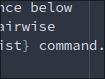
\includegraphics[width=0.7\textwidth]{figures/image.png}
  \caption{Sketch counts for sequence XYZ of Phytophthora infestans}
  \label{fig:sketchCountsOverview}
\end{figure}

\subsection*{Windows with unusual hash counts can be linked to low sequence complexity}
Looking at the plot for sequence complexity in
Figure~\ref{fig:sketchCountsOverview}, one could hypothyse that windows with
unusual hash counts also have a low sequence complexity. When mapping the hash
counts per window to the sequence complexity of that window, we can observe that
for many genome sequences, windows with unusual hash counts have significantly
lower complexity values (Table~\ref{ta:hashCountComplexity}).

% Please add the following required packages to your document preamble:
% \usepackage{booktabs}
\begin{longtable}{@{}lrrrrr@{}}
  \toprule
  \textbf{}                           & $\textbf{$n$}$ & \textbf{$u$} & \textbf{$r$} & \textbf{$z$} & \textbf{$p$}  \\ \midrule
  \endhead
  \textit{P. x alni}                  & 61         & 0          & 0.1170       &              &               \\
  \textit{P. cambivora}               & 727        & 0          & -0.0272      &              &               \\
  \textit{P. cryptogea}               & 1922       & 0          & -0.038       &              &               \\
  \textit{P. lateralis}               & 2438       & 0          & 0.0089       &              &               \\
  \textit{P. pinifolia}               & 1492       & 0          & -0.0139      &              &               \\
  \textit{P. rubi}                    & 4951       & 34         & 0.1661       & 586.0        & 1.6328e-23    \\
  \textit{P. multivora}               & 2908       & 0          & 0.0357       &              &               \\
  \textit{P. podocarpi}               & 3754       & 0          & 0.0144       &              &               \\
  \textit{P. pluvialis}               & 3594       & 0          & 0.0038       &              &               \\
  \textit{P. megakarya}               & 2738       & 0          & 0.0255       &              &               \\
  \textit{P. litchii}                 & 2676       & 0          & 0.0027       &              &               \\
  \textit{P. citricola}               & 4976       & 60         & 0.1617       & 2423.0       & 2.7069e-39   \\
  \textit{P. palmivora}               & 15371      & 220        & 0.239        & 31064.5      & 2.9029e-138 \\
  \textit{P. kernoviae}               & 3921       & 12         & 0.1693       & 584.0        & 5.19523e-09   \\
  \textit{P. fragariae}               & 9314       & 61         & 0.1389       & 9175.0       & 6.8477e-39    \\
  \textit{P. betacei}                 & 26688      & 437        & 0.2446       & 180086.0     & 4.5575e-265  \\
  \textit{P. macrochlamydospora}      & 6548       & 84         & 0.2809       & 5098.5       & 5.12064e-54   \\
  \textit{P. constricta}              & 7631       & 56         & 0.2304       & 3508.0       & 5.9580e-37  \\
  \textit{P. quininea}                & 8237       & 92         & 0.2095       & 8577.5       & 1.3136e-58  \\
  \textit{P. boehmeriae}              & 5002       & 51         & 0.2252       & 2396.5       & 1.4980e-33  \\
  \textit{P. chlamydospora}           & 2525       & 0          & 0.0625       &              &              \\
  \textit{P. gonapodyides}            & 602        & 0          & -0.053       &              &              \\
  \textit{P. hibernalis}              & 8253       & 232        & 0.3493       & 17987.0      & 1.7783e-143  \\
  \textit{P. syringae}                & 7178       & 83         & 0.2394       & 5617.5       & 1.9746e-53  \\
  \textit{P. quercina}                & 7118       & 262        & 0.2486       & 59409.0      & 1.3955e-145 \\
  \textit{P. castanetorum}            & 6928       & 295        & 0.2282       & 43430.5      & 2.8891e-170  \\
  \textit{P. ohioensis}               & 7305       & 221        & 0.0325       & 35095.0      & 1.4426e-129 \\
  \textit{P. tubulina}                & 7539       & 223        & 0.4525       & 17186.0      & 2.6610e-137  \\
  \textit{P. sp. ST\_20190627}        & 7433       & 310        & 0.1582       & 67520.5      & 7.9153e-173  \\
  \textit{P. vignae}                  & 8337       & 62         & 0.1548       & 8252.0       & 1.7135e-39  \\
  \textit{P. cactorum}                & 6501       & 8          & 0.0069       & 296.0        & 1.3003e-06  \\
  \textit{P. idaei}                   & 4468       & 0          & 0.0179       &              &                         \\
  \textit{P. cinnamomi}               & 10799      & 28         & -0.0933      & 3720.0       & 4.3767e-19  \\
  \textit{P. colocasiae}              & 9197       & 137        & 0.1783       & 38087.0      & 1.4964e-79  \\
  \textit{P. aleatoria}               & 3200       & 0          & 0.0155       &              &                         \\
  \textit{P. pseudosyringae}          & 3414       & 0          & -0.0158      &              &                         \\
  \textit{P. ramorum}                 & 5671       & 51         & 0.1791       & 4882.5       & 1.2873e-32  \\
  \textit{P. pini}                    & 5115       & 169        & 0.1786       & 10634.5      & 3.0103e-103   \\
  \textit{P. melonis}                 & 10456      & 97         & 0.1958       & 20345.0      & 1.1427e-59  \\
  \textit{P. brassicae}               & 2994       & 0          & 0.0289       &              &             \\
  \textit{P. uliginosa}               & 1909       & 0          & 0.0422       &              &             \\
  \textit{P. pistaciae}               & 2148       & 0          & -0.0177      &              &             \\
  \textit{P. foliorum}                & 2392       & 0          & -0.0239      &              &             \\
  \textit{P. cajani}                  & 854        & 0          & 0.0142       &              &             \\
  \textit{P. pisi}                    & 2857       & 0          & 0.0142       &              &             \\
  \textit{P. niederhauseri}           & 1009       & 0          & -0.026       &              &             \\
  \textit{P. parvispora}              & 877        & 0          & 0.0148       &              &             \\
  \textit{P. agathidicida}            & 5687       & 109        & 0.2133       & 23970.5      & 3.9572e-61  \\
  \textit{P. plurivora}               & 4630       & 51         & 0.0497       & 2432.5       & 2.0990e-33   \\
  \textit{P. lilii}                   & 3462       & 0          & -0.0024      &              &                         \\
  \textit{P. fragariaefolia}          & 4841       & 0          & -0.0008      &              &                         \\
  \textit{P. capsici}                 & 7774       & 395        & 0.3854       & 78063.0      & 4.4484e-221  \\
  \textit{P. europaea}                & 2243       & 0          & -0.0025      &              &                         \\
  \textit{P. citrophthora}            & 4760       & 141        & 0.2145       & 9332.0       & 3.3680e-86   \\
  \textit{P. sansomeana}              & 7256       & 103        & 0.3111       & 17233.0      & 3.8511e-62   \\
  \textit{P. meadii}                  & 5241       & 0          & 0.0032       &              &                         \\
  \textit{P. tentaculata}             & 10896      & 566        & 0.3496       & 178552.5     & 1.5395e-310   \\
  \textit{P. x cambivora}             & 15079      & 332        & 0.2247       & 242342.5     & 5.6589e-174  \\
  \textit{P. crassamura}              & 7920       & 203        & 0.2312       & 57354.0      & 7.7190e-113  \\
  \textit{P. taxon juncus}            & 6456       & 379        & 0.2364       & 143692.5     & 2.8069e-180  \\
  \textit{P. sp. 'mugwort'}           & 8562       & 189        & 0.1093       & 55262.5      & 2.5058e-106  \\
  \textit{P. infestans}               & 11173      & 37         & 0.1830       & 6904.5       & 2.8352e-24   \\
  \textit{P. sojae}                   & 7339       & 74         & 0.1570       & 5092.0       & 6.5134e-48    \\
  \textit{P. nicotianae}              & 2529       & 0          & -0.0042      &              &                         \\ \bottomrule
  
  \caption{Results of the analysis of windows with size $w=10000$ with unusual
  hash counts. $n$ is the total number of windows analyzed for a genome
  (excluding windows with ambiguous bases, that is, windows with $C_m=-1$). $u$
  is the number of windows with unusual hash counts. $r$ is the Pearson
  correlation cofficient of hash count and complexity in a window. $z$ and $p$
  are the results of the Mann-Whitney-U test performed, missing values indicate
  that no test was performed because of $u=0$.}
  \label{ta:hashCountComplexity}
\end{longtable}

\subsection*{Windows with unusual hash counts do not contain CDS}
Given that there is evidence for the "Two Speeds genome" hypothesis in
\textit{Phytophthora infestans} \cite{dongTwospeedGenomesFilamentous2015}, it is
interesting to check if there are genes coding for effector preoteins located in
some of the windows with unusual hash counts. However, there is not a single CDS
in those windows and therefore also no CDS coding for effector proteins.


\section{\texttt{fmhdist} is slower than \texttt{mash} and \texttt{sourmash}}
The results of the performance analysis are listed in
Table~\ref{ta:performance}. The dataset has a combined size of $5.477$ GBp,
so \texttt{fmhdist} is capable of sketching $\approx 26$ MBp/s using a single
thread and $\approx 65$ MBp/s using six threads. This is outperformed
drastically by \texttt{mash}, which is capable of sketching $\approx 40$ MBp/s
and $\approx 107$ MBp/s. \texttt{sourmash} ($\approx 31$ MBp/s) is faster than
\texttt{fmhdist} but slower than \texttt{mash} using a single core, but is not
offering multithreading out of the box. 

\begin{table}[]
  \centering
  \begin{tabular}{@{}lrrrrr@{}}
  \toprule
                  & \texttt{mash} (1)     & \texttt{mash} (6) & \texttt{sourmash} (1) & \texttt{fmhdist} (1) & \texttt{fmhdist} (6) \\ \midrule
  min (s) & 135                     &  44                     &  171              &  201                      & 75                         \\
  max (s) & 140                     &  58                     &  178              &  215                      & 91                         \\
  avg (s) & 137                     &  51                     &  174              &  208                      & 84                         \\ \bottomrule
  \end{tabular}
  \caption{Runtime comparison of \texttt{mash}, \texttt{sourmash} and
  \texttt{sourmash} to calculate sketches for dataset C. The number of threads used is stated in parantheses.}
  \label{ta:performance}
\end{table}

\clearpage
